

\begin{figure}[bt]
    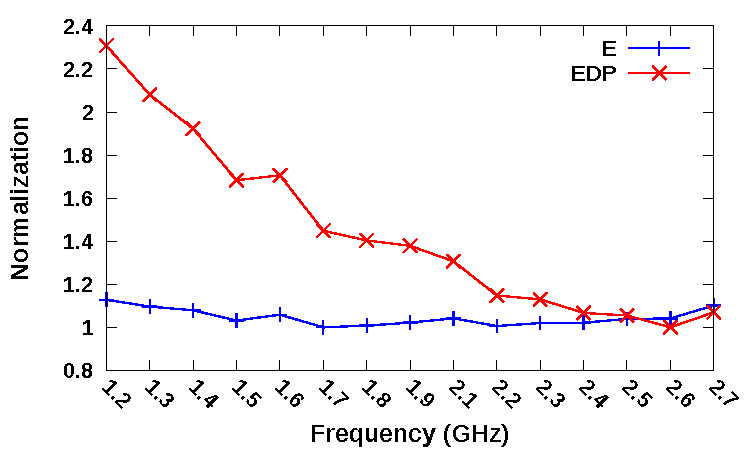
\includegraphics[width=3.in]{dvfs-all}
%    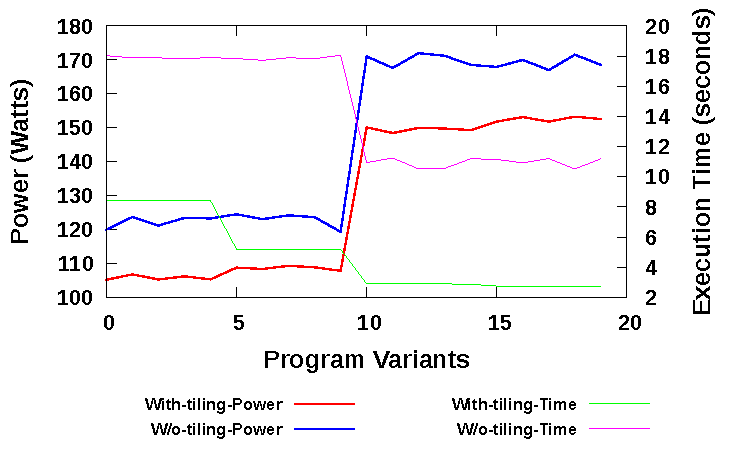
\includegraphics{Covariance}
    \caption{Graph showing the normalized Energy(E)/EDP by varying the frequency. The minimum E/EDP is chosen as
the baseline.}
    \label{fig:cdc-fs}
\end{figure}

Figure 2-4 shows that three different loops inside the same application 
achieve minimum energy at different frequency scaling setting and duty cycle modulation setting.
For example, in Figure 2(a), the minimum energy is achieved by operating the processsor 
at a frequency 1.6GHz. In Figure 2(b), the minimum energy is achieved by setting duty cycle
modulation level to be 9, i.e. let the cores be active for 56.25\% (=9/16) of the time.

We then let the three loops run with the frequency setting of 1.6GHz, 2.4GHz,
2.7GHz respectively and recorded the time and energy of the hybrid version.
We also ran the three loops with the duty cycle modulation level of 9, 15, 16 respectively.

Table 1 compares the two runs with the minimum energy runs achieved by
 coarse-grained DVFS and DCM (i.e. presetting a fixed DVFS/DCM level and running the 
whole program with the preset configuration). We can see that coarse-grained DVFS 
achieved the minimum energy, the fine-grained DVFS consumed the maximum energy.
Fine-grained DCM reduced energy consumption compared with coarse-grained DCM. 
This table tell us that DCM can be used in fine-grained loops and DVFS can 
be more effective than DCM for coarse-grained (large) loops.
%We also compare the two runs 
%with the minimum time runs achieved by coarse-grained DVFS and DCM, shown in the third column of Table 1.  


\begin{table}[!ht]
  \centering{
\caption{Time and Energy Comparison of Optimal Configuration to Baseline of Polybench Kernels on SandyBridge}
\begin{tabular}{ |l|c|c|c|c| }
  \hline
  \multirow{2}{*}{\textbf{Metrics}} & \multicolumn{2}{|c|}{\textit{Coarse-Grain}} & \multicolumn{2}{|c|}{\textit{Fine-Grain}} \\
  \cline{2-5}
  & DVFS & DCM & DVFS & DCM \\
  \hline
  Time & 26.47 & 24.54 & 26.86 & 26.74 \\
  \hline
  Energy & \textcolor{green}{1647} & 1701 & \textcolor{red}{1728.23} & 1682 \\
  \hline
  Power & 62.23 & 69.33 & 64.34 & 62.80 \\
  \hline
\end{tabular}
  }
  \label{SandyTable}
\end{table}





\begin{figure*}[bt]
\centering
\subfigure[Frequency Scaling Energy and Energy-Delay Product (Normalized) of the Loop] {
  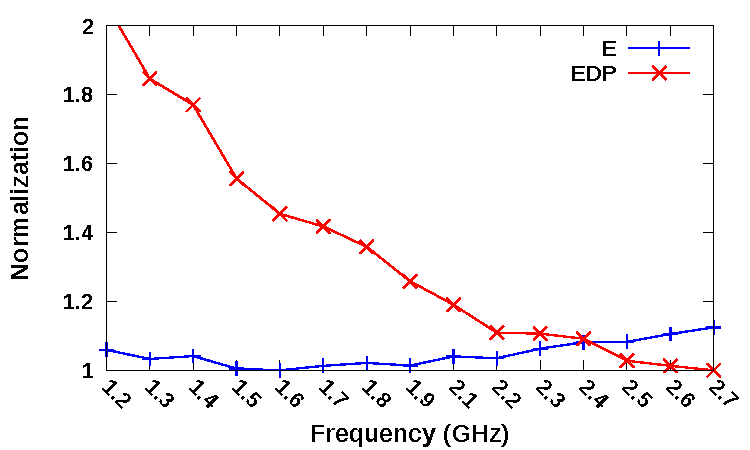
\includegraphics[width=0.45\textwidth]{fs-13}
  \label{fs-13}
}
\subfigure[Duty Cycle Modulation Energy and Energy-Delay Product (Normalized Values over 2 are Omitted) of the Loop] {
  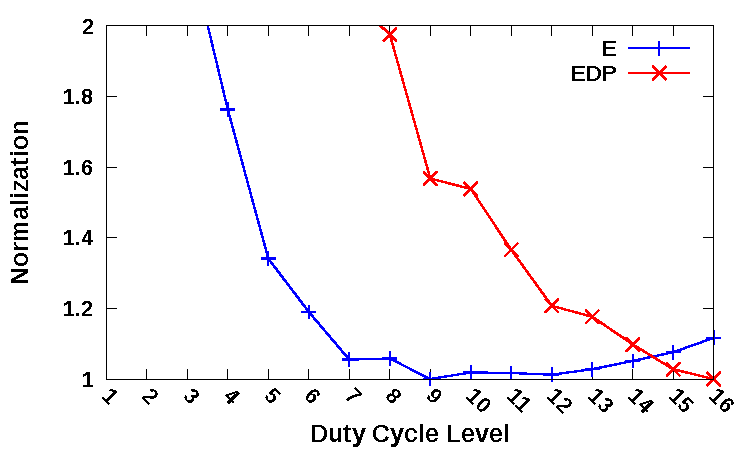
\includegraphics[width=0.45\textwidth]{dc-13}
  \label{dc-13}
}
\caption{Graph showing the energy (E) and energy-delay product (EDP) of the 1st loop
by varing frequency and changing duty cycle modulation. Minimal E are achieved at 1.6GHz for DVFS and level 9 (56.25\% active) for DCM. 
Minimal EDP are achieved at maximum settings for both DVFS and Duty Cycle Modulation. These minimal E and EDP are the baselines for normalization.}
\label{fig:Brdr2d-TE}
\end{figure*}

\begin{figure*}[bt]
\centering
\subfigure[Frequency Scaling Energy and Energy-Delay Product (Normalized Values over 2 are Omitted) of the Loop] {
  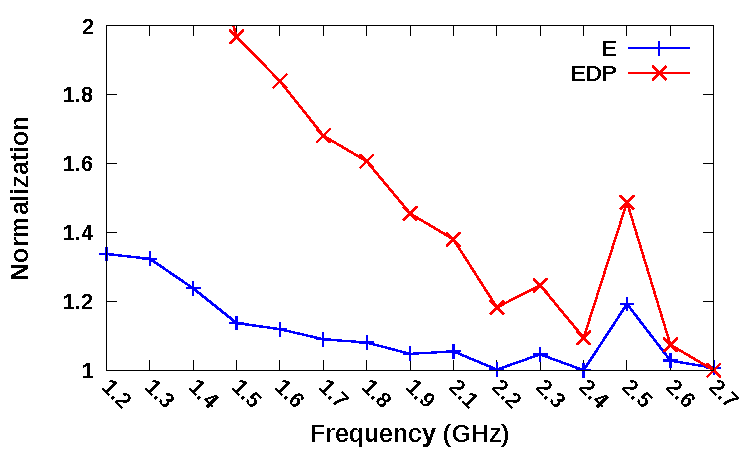
\includegraphics[width=0.45\textwidth]{fs-14}
  \label{fs-14}
}
\subfigure[Duty Cycle Modulation Energy and Energy-Delay Product (Normalized Values over 2 are Omitted) of the Loop] {
  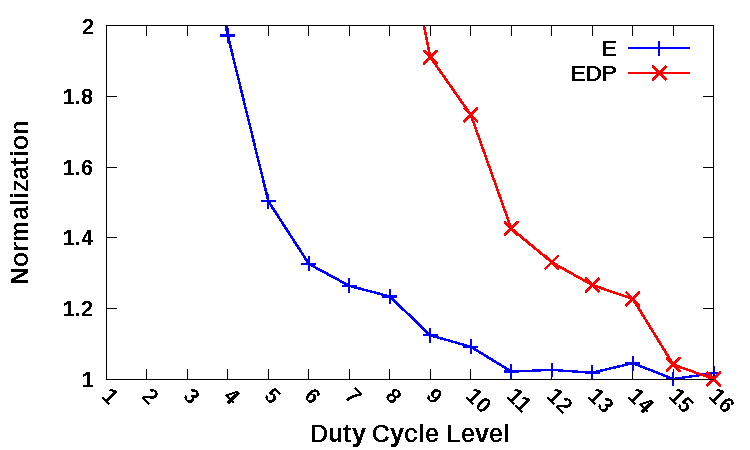
\includegraphics[width=0.45\textwidth]{dc-14}
  \label{dc-14}
}
\caption{Graph showing the energy (E) and energy-delay product (EDP) of the 2nd loop
by varing frequency and changing duty cycle modulation. Minimal E are achieved at 2.4GHz for DVFS and 
level 15 (93.75\% active) for DCM. Minimal EDP are achieved at maximum settings for both DVFS and Duty Cycle Modulation. These minimal E and EDP are the baselines for normalization.}
\label{fig:Brdr2d-TE}
\end{figure*}

\begin{figure*}[bt]
\centering
\subfigure[Frequency Scaling Energy and Energy-Delay Product (Normalized Values over 2 are Omitted) of the Loop] {
  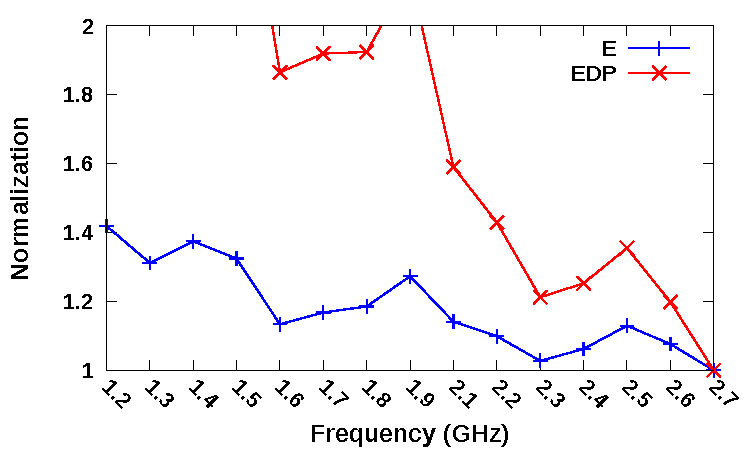
\includegraphics[width=0.45\textwidth]{fs-16}
  \label{fs-16}
}
\subfigure[Duty Cycle Modulation Energy and Energy-Delay Product (Normalized Values over 2 are Omitted) of the Loop] {
  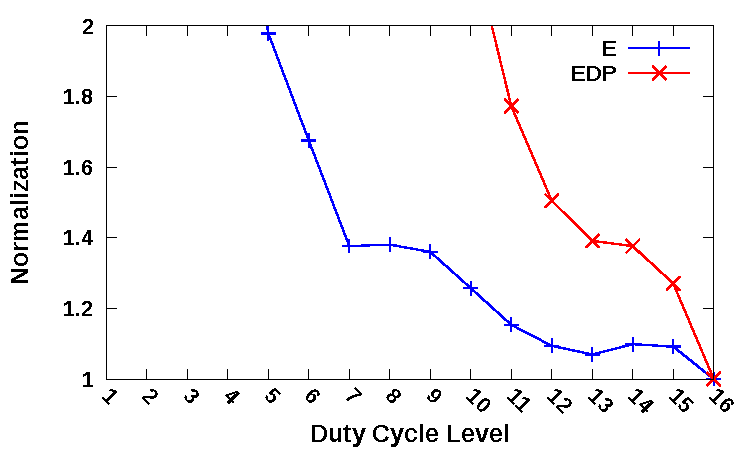
\includegraphics[width=0.45\textwidth]{dc-16}
  \label{dc-16}
}
\caption{Graph showing the energy (E) and energy-delay product (EDP) of the 3rd loop
by varing frequency and changing duty cycle modulation. Minimal E and minimal EDP 
are at maximum settings for both DVFS and Duty Cycle Modulation. These minimal E and EDP are the baselines for normalization.}
\label{fig:Brdr2d-TE}
\end{figure*}
